\documentclass[10pt,utf8]{beamer}
\usepackage[utf8]{inputenc}
\usepackage[russian]{babel}

% \usepackage{lmodern}
\usetheme{Dresden}
\usecolortheme{beaver}
% \useoutertheme{shadow}

\definecolor{links}{HTML}{2A1B81}
\hypersetup{colorlinks,linkcolor=,urlcolor=links}

\title{Немного о ReactJS}
\date{Донецкий Lambda-клуб. 31 мая 2014}
\author{Андрей Кутейко}

\begin{document}

\begin{frame}
  \titlepage
\end{frame}

\begin{frame}[fragile]
  \frametitle{Простейшее приложение}
  \framesubtitle{Рендеринг}

  \begin{semiverbatim}
    <!DOCTYPE html>
    <div id='app'></div>
    <script>
    React.renderComponent(
      React.DOM.a(\{href: 'http://lambda.dn.ua'\}, 'Click me'),
      document.getElementById('app'));
    </script>
  \end{semiverbatim}
\end{frame}

\begin{frame}[fragile]
  \frametitle{Простейшее приложение}
  \framesubtitle{Класс}

  \begin{semiverbatim}
    var SimpleApp = React.createClass(\{
      render: function() \{
        \alert{return React.DOM.a(
          \{href: 'http://lambda.dn.ua'\},
          'Click me'
        );}
      \}
    \});

    React.renderComponent(
      \alert{SimpleApp()},
      document.getElementById('app'));
  \end{semiverbatim}
\end{frame}

\begin{frame}[fragile]
  \frametitle{Простейшее приложение}
  \framesubtitle{Свойства}

  \begin{semiverbatim}
    var SimpleApp = React.createClass(\{
      render: function() \{
        return React.DOM.a(
          \{href: \alert{this.props.url}\},
          \alert{this.props.title}
        );
      \}
    \});

    React.renderComponent(
      SimpleApp(\alert{\{url: 'http://l.dn.ua', title: 'Жми!'\}}),
      document.getElementById('app'));
  \end{semiverbatim}
\end{frame}

\begin{frame}[fragile]
  \frametitle{Простейшее приложение}
  \framesubtitle{Ссылки и события}

  \begin{semiverbatim}
    var SimpleApp = React.createClass(\{
      render: function() \{
        return React.DOM.div(null,
          React.DOM.input(\{\alert{ref: 'inp'}\}),
          React.DOM.a(
            \{href: '', onClick: \alert{this.onClick}\},
            this.props.title
          )
        );
      \},
      onClick: function(event) \{
        event.preventDefault();
        document.location = \alert{this.refs.inp.getDOMNode()}.value;
      \}
    \});
  \end{semiverbatim}
\end{frame}

\begin{frame}[fragile]
  \frametitle{Простейшее приложение}
  \framesubtitle{Компонент}

  \fontsize{9pt}{9.2}\selectfont

  \begin{semiverbatim}
    var \alert{Button} = React.createClass(\{
      getDefaultProps: function() \{
        return \{ title: 'Button1',
                 onClick: function() \{\} \};
      \},
      render: function() \{
        React.DOM.a(\{ href: '',
                      className: 'btn',
                      onClick: this.onClick\},
          this.props.title);
      \},
      onClick: function(event) \{
        event.preventDefault();
        this.props.onClick();
      \}
    \});
  \end{semiverbatim}
\end{frame}

\begin{frame}[fragile]
  \frametitle{Простейшее приложение}
  \framesubtitle{Компонент (cont.)}

  \begin{semiverbatim}
    var SimpleApp = React.createClass(\{
      render: function() \{
        return React.DOM.div(null,
          React.DOM.input(\{ref: 'inp'\}),
          \alert{Button(\{ title: this.props.title,
                   onClick: \alert{this.onButtonClick} \})}
        );
      \},
      onButtonClick: function() \{
        document.location = this.refs.inp.getDOMNode().value;
      \}
    \});
  \end{semiverbatim}
\end{frame}

\begin{frame}[fragile]
  \frametitle{Простейшее приложение}
  \framesubtitle{Состояние}

  \fontsize{9pt}{9.2}\selectfont

  \begin{semiverbatim}
    var SimpleApp = React.createClass(\{
      getInitialState: function() \{
        return \{ \alert{url: ''} \};
      \},
      render: function() \{
        return React.DOM.div(null,
          React.DOM.input(\{ onChange: this.onUrlChange,
                            value: \alert{this.state.url} \}),
          Button(\{ onClick: this.onButtonClick \})
        );
      \},
      onUrlChange: function(event) \{
        \alert{this.setState(\{url: event.target.value\});}
      \},
      onButtonClick: function(event) \{
        document.location = \alert{this.state.url};
      \}
    \});
  \end{semiverbatim}
\end{frame}

\begin{frame}[fragile]
  \frametitle{Простейшее приложение}
  \framesubtitle{Состояние}

  \begin{semiverbatim}
    var CounterApp = React.createClass(\{
      getInitialState: function() \{
        return \{ \alert{count: 0} \};
      \},
      render: function() \{
        return Button(
          \{ onClick: this.onClick \},
          \alert{this.state.count}
        );
      \},
      onClick: function() \{
        this.setState(\{\alert{count: this.state.count + 1}\});
      \}
    \});
  \end{semiverbatim}
\end{frame}

\begin{frame}[fragile]
  \frametitle{Простейшее приложение}
  \framesubtitle{Data flow}

  $$ (props \times state) \rightarrow Virtual DOM \rightarrow DOM $$

  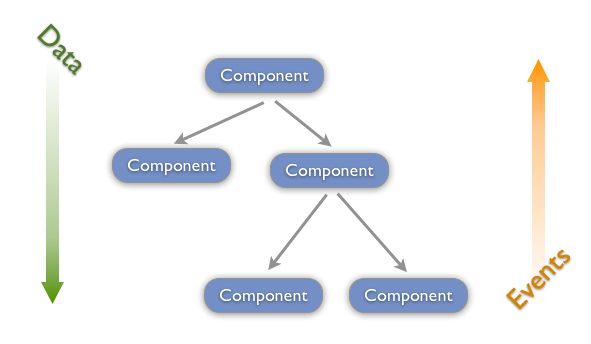
\includegraphics[scale=0.5]{data-event-flow.png}
\end{frame}

\begin{frame}[fragile]
  \frametitle{Простейшее приложение}
  \framesubtitle{Компонентам состояние не нужно}

  \fontsize{9pt}{9.2}\selectfont

  \begin{semiverbatim}
    var List = React.createClass(\{
      render: function() \{
        return React.DOM.ul(null,
          this.props.children.map(function(item, index) \{
            return React.DOM.div(null,
              item,
              Button(\{onClick: this.onDelete.curry(index)\}, 'Delete')
            );
          \}, this)
        );
      \},
      onDelete: function(index) \{
        this.props.onDeleteItem(index);

        // ИЛИ

        var children = this.props.children.slice(0).splice(index, 1);
        this.props.onChangeChildren(children);
      \}
    \});
  \end{semiverbatim}
\end{frame}

\begin{frame}[fragile]
  \frametitle{Простейшее приложение}
  \framesubtitle{Миксины}

  \fontsize{9pt}{9.2}\selectfont

  \begin{semiverbatim}
var UndoStack = \{
  getInitialState: function() \{
    return \{ undo: [] \};
  \},
  snapshot: function() \{
    var undo = this.state.undo.concat(\alert{this.getStateSnapshot()});
    this.setState(\{ undo: undo \});
  \},
  undo: function() \{
    var undo = this.state.undo.slice(0);
    var snapshot = undo.pop();
    \alert{this.setStateSnapshot(snapshot)};
    this.setState(\{ undo: undo \});
  \}
\};

var MyComponent = React.createClass(\{
  mixins: [ UndoStack ],
  getStateSnapshot: function() \dots
  setStateSnapshot: function(snapshot) \dots
  \end{semiverbatim}
\end{frame}

\begin{frame}[fragile]
  \frametitle{Жизненный цикл компонентов}

  \begin{itemize}
  \item Вставка (mounting)

    getInitialState \\
    componentWillMount \\
    componentDidMount

    \pause

  \item Обновление (updating)

    componentWillReceiveProps \\
    shouldComponentUpdate \\
    componentWillUpdate \\
    componentDidUpdate

    \pause

  \item Удаление (unmounting)

    componentWillUnmount
  \end{itemize}
\end{frame}

\begin{frame}[fragile]
  \frametitle{JSX}

  \fontsize{9pt}{9.2}\selectfont

  \begin{semiverbatim}
    /** @jsx React.DOM */

    var SimpleApp = React.createClass(\{
      \dots
      render: function() \{
        return \alert{<div>
          <input onChange=}\{this.onUrlChange\} \alert{value=}\{this.state.url\}\alert{>
          <Button onClick=}\{this.onButtonClick\}\alert{>
        </div>;}
      \},
      \dots
    \});
  \end{semiverbatim}
\end{frame}

\begin{frame}[fragile]
  \frametitle{Разное}

  \begin{itemize}
  \item Синтетические события
    \pause
  \item Server-side rendering
    \pause
  \item SVG, Canvas\dots
    \pause
  \item Тестируемость $(props \times state) \rightarrow Virtual DOM$
  \end{itemize}
\end{frame}

\begin{frame}[fragile]
  \frametitle{Ссылки}

  \begin{enumerate}
  \item \href{http://facebook.github.io/react/}{http://facebook.github.io/react/}
  \item \href{https://github.com/andy128k/reactjs-presentation}{https://github.com/andy128k/reactjs-presentation}
  \end{enumerate}
\end{frame}

\end{document}

